%%%%%%%%%%%%%%%%%%%%%%%%%%%%%%%%%%%%%%%%%%%%%%%%%%%%%%%%%%%%%%%%%%%%%%%%%%%%%%%%%%%%%%%%%%%%%%%%%%%%%%%%%%%
%   \copyright 2013 Ricardo García Fernández - ricardogarfe [at] gmail [dot] com.
%
%    This work is licensed under a Creative Commons 3.0 Unported License.
%    To view a copy of this license visit:
% 
%    http://creativecommons.org/licenses/by/3.0/legalcode
%%%%%%%%%%%%%%%%%%%%%%%%%%%%%%%%%%%%%%%%%%%%%%%%%%%%%%%%%%%%%%%%%%%%%%%%%%%%%%%%%%%%%%%%%%%%%%%%%%%%%%%%%%

%%%%%%%%%%%%%%%%%%%%%%%%%%%%%%%%%%%%%%%%%%%%%%%%%%%%%%%%%%%%%%%%%%%%%%%%%%%%%%%%%%%%%%%%%%%%%%%%%%%%%%%%%%
% SCStack
%%%%%%%%%%%%%%%%%%%%%%%%%%%%%%%%%%%%%%%%%%%%%%%%%%%%%%%%%%%%%%%%%%%%%%%%%%%%%%%%%%%%%%%%%%%%%%%%%%%%%%%%%%

\chapter{SCStack}
\label{chap:scstack}

\par SCStack es el conjunto de herramientas que componen la Forja de desarrollo. La palabra \emph{stack} en Inglés significa \emph{pila}, con respecto a la forja se trata del conjunto de herramientas apiladas y conectadas que dan forma a la Forja.

\begin{figure}[H]
    \centering
    
\includegraphics[width=0.7\textwidth]{stackstorage}
    \caption{Ejemplo de pila a partir de cajones}
    \label{fig:stackstorage}
\end{figure}

\section{Arquitectura}
\label{sec:arquitectura}

\par La arquitectura del Sistema de Gestión de la Forja se ve reflejada en el siguiente esquema:

\begin{figure}[H]
    \centering
    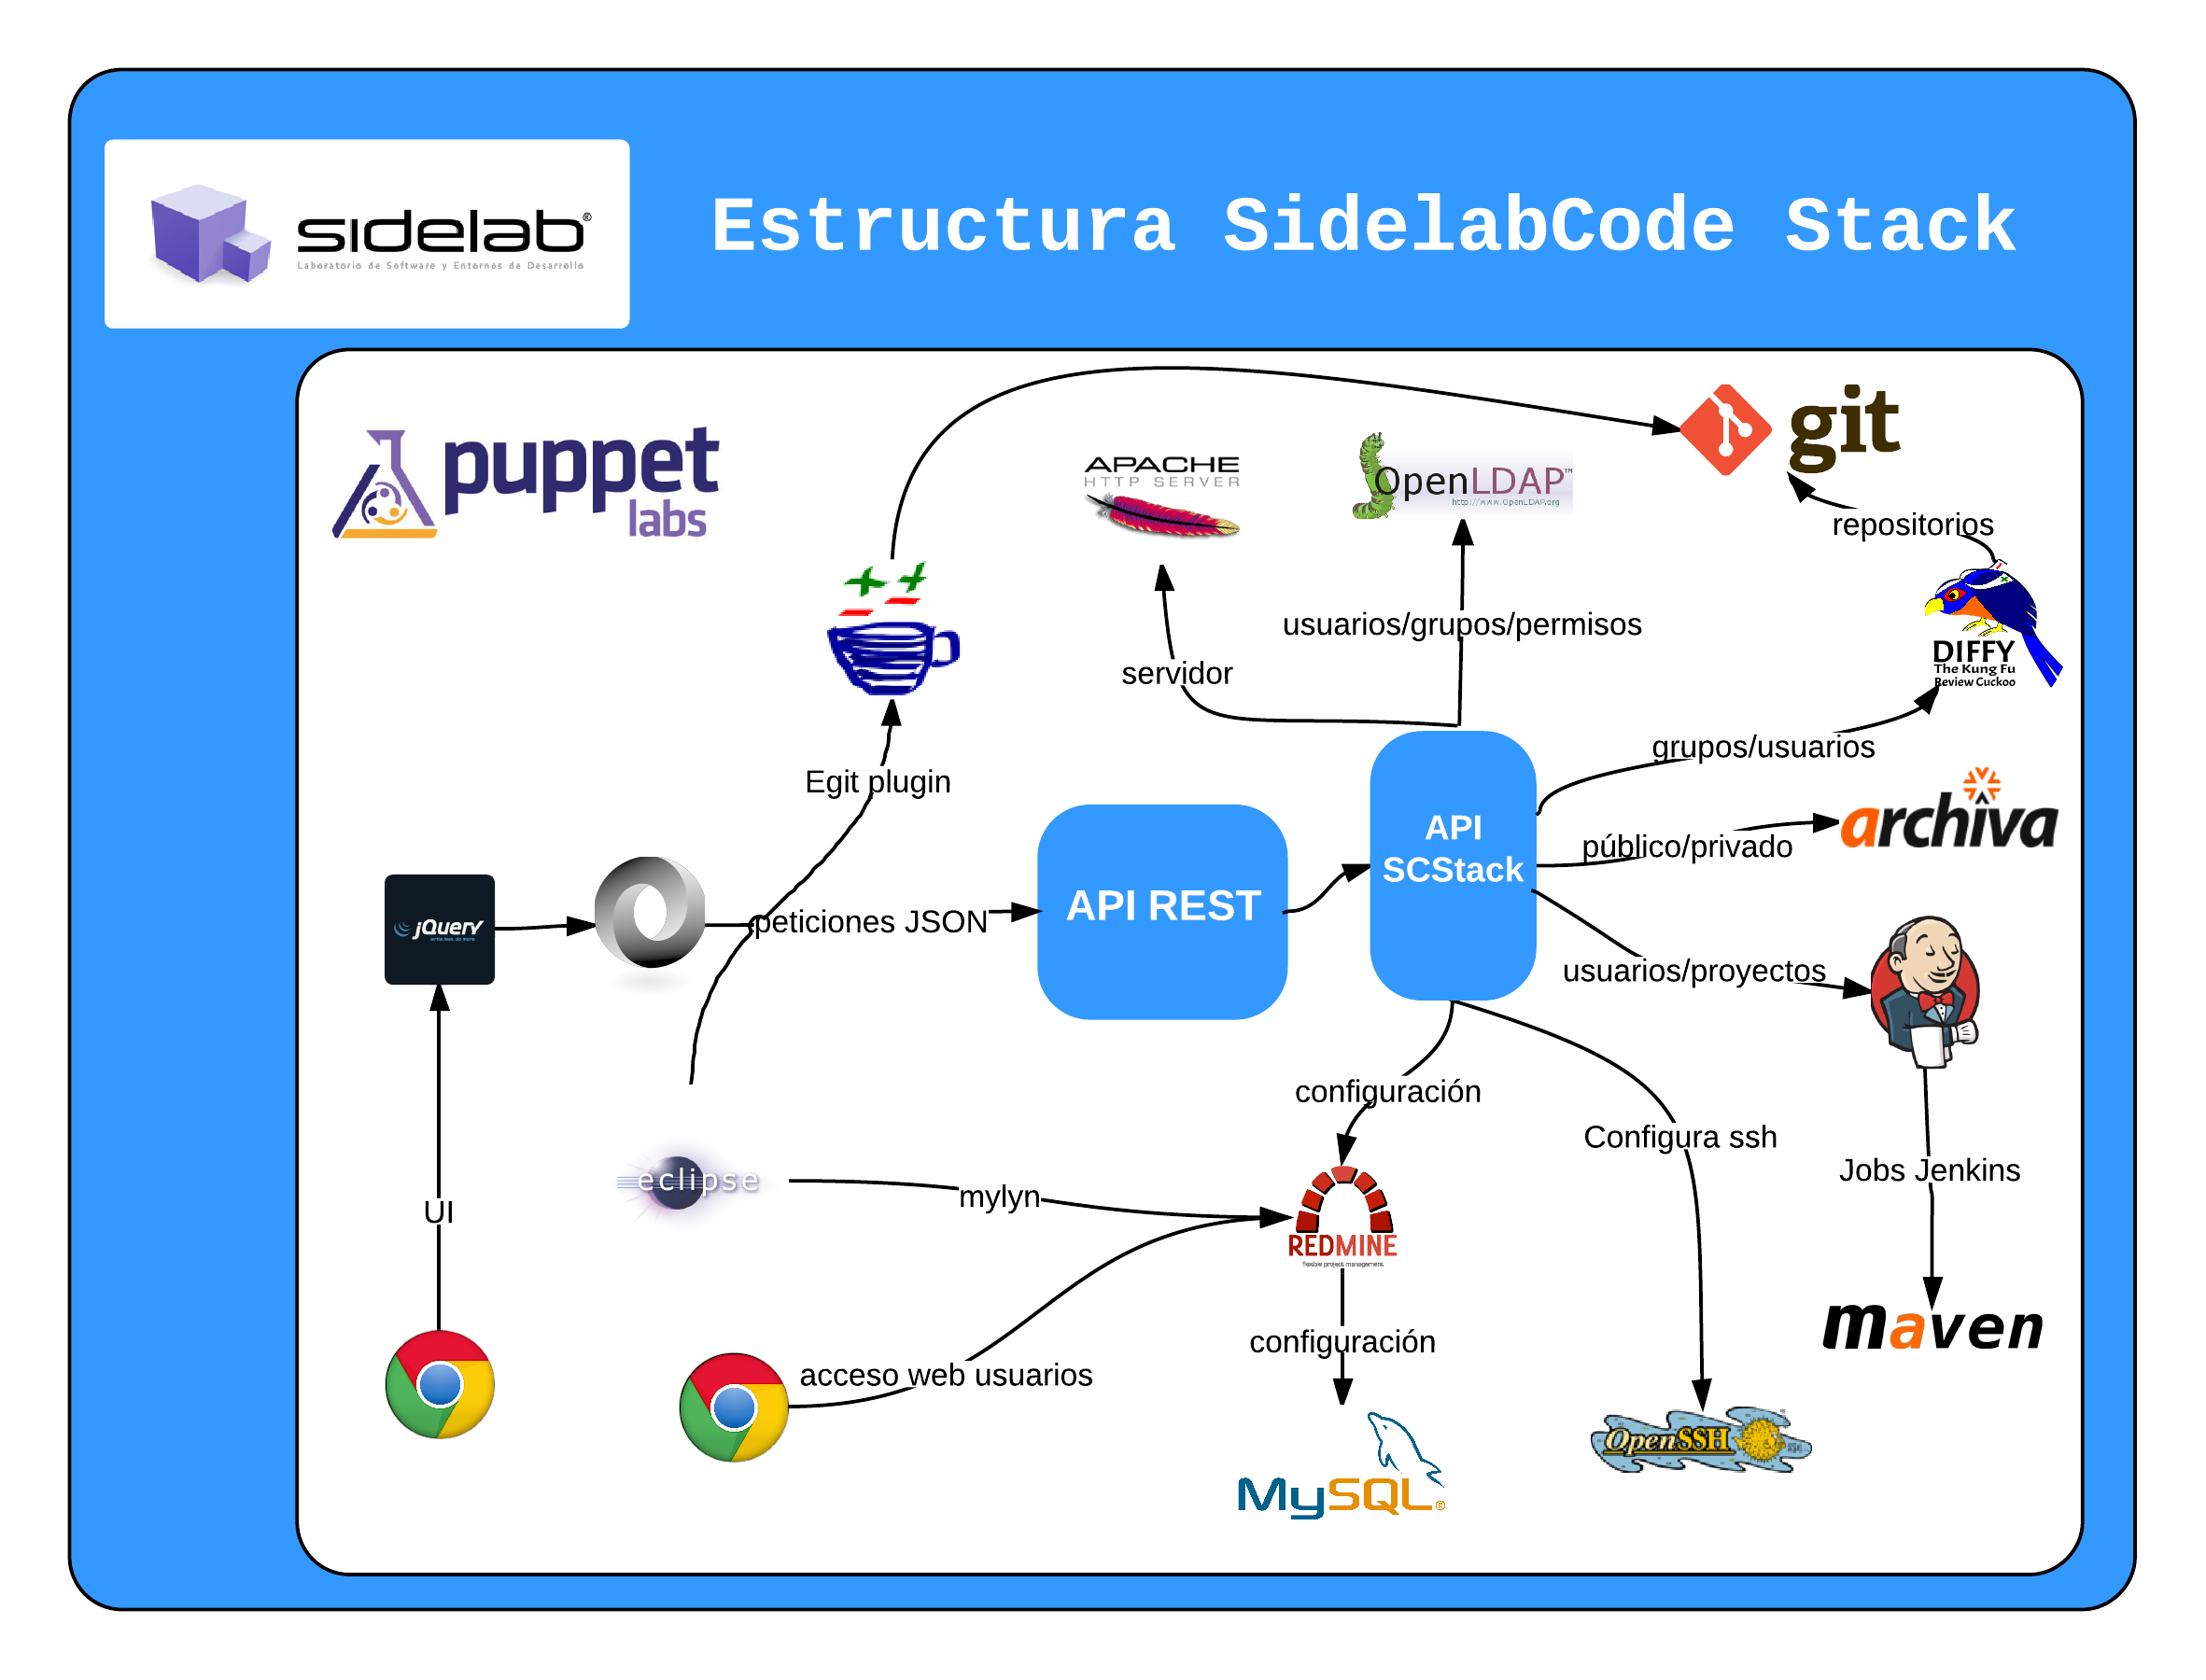
\includegraphics[width=\textwidth]{scstack-diagram}
    \caption{Diagrama de arquitectura SCStack}
    \label{fig:scstack-diagram}
\end{figure}

\par El proyecto consta de tres componentes conectados entre sí para la comunicación del usuario con las herramientas para la gestión de los proyectos: La Consola de Administración, el servidor de servicios web REST y el API.

%%%%%%%%%%%%%%%%%%%%%%%%%%%%%%%%%%%%%%%%%%%%%%%%%%%%%%%%%%%%%%%%%%%%%%%%%%%%%%%%%%%%%%%%%%%%%%%%%%%%%%%%%%
% Consola de Administración
%%%%%%%%%%%%%%%%%%%%%%%%%%%%%%%%%%%%%%%%%%%%%%%%%%%%%%%%%%%%%%%%%%%%%%%%%%%%%%%%%%%%%%%%%%%%%%%%%%%%%%%%%%

\subsection{Consola de Administración}
\label{sub:consola-admin}

\par \textbf{Consola de Administración}: Se trata de la capa de la vista encargada de interactuar con el usuario. A través de la interfaz que se ejecuta sobre un navegador web, el usuario administrador gestiona los usuarios y los proyectos de la Forja: crear, editar, modificar, eliminar y buscar), el típico sistema CRUD-F\footnote{\url{http://en.wikipedia.org/wiki/Create,\_read,\_update\_and\_delete}} (\emph{CRUD: Create, Read, Update and Delete also Find}). Está diseñada con el framework Javascript \emph{jQuery} por lo que no requiere ninguna librería externa para su uso, únicamente el navegador del cliente. Las operaciones que se realizan en la capa UI se trasladan al servidor REST a través de peticiones \emph{http} asíncronas mediante las interfaces REST definidas.

% subsection consola-admin (end)

%%%%%%%%%%%%%%%%%%%%%%%%%%%%%%%%%%%%%%%%%%%%%%%%%%%%%%%%%%%%%%%%%%%%%%%%%%%%%%%%%%%%%%%%%%%%%%%%%%%%%%%%%%
% Servicio web REST
%%%%%%%%%%%%%%%%%%%%%%%%%%%%%%%%%%%%%%%%%%%%%%%%%%%%%%%%%%%%%%%%%%%%%%%%%%%%%%%%%%%%%%%%%%%%%%%%%%%%%%%%%%

\subsection{Servicio web REST}
\label{sub:rest-ws}

\par \emph{REST}: Representational State Transfer se trata de una arquitectura acuñada por \emph{Roy Fielding}\footnote{\url{http://roy.gbiv.com/}}, uno de los autores de la especificación del protocolo \emph{HTTP}. Esta arquitectura de comunicación se basa en cuatro principios:

\begin{itemize}
	\item Un protocolo cliente/servidor \emph{sin estado}: cada mensaje HTTP contiene toda la información necesaria para comprender la petición. Como resultado, ni el cliente ni el servidor necesitan recordar ningún estado de las comunicaciones entre mensajes. Sin embargo, en la práctica, muchas aplicaciones basadas en HTTP utilizan cookies y otros mecanismos para mantener el estado de la sesión.

	\item Un \emph{conjunto de operaciones} bien definidas que se aplican a todos los recursos de información: HTTP en sí define un conjunto pequeño de operaciones, las más importantes son \textbf{POST}, \textbf{GET}, \textbf{PUT} y \textbf{DELETE}.

	\item Una sintaxis \emph{universal} para identificar los recursos. En un sistema REST, cada recurso es direccionable únicamente a través de su URI.

	\item El uso de \emph{hipermedios}: tanto para la información de la aplicación como para las transiciones de estado de la aplicación. Como resultado de esto, es posible navegar de un recurso REST a muchos otros, simplemente siguiendo enlaces sin requerir el uso de registros u otra infraestructura adicional.
\end{itemize}

\par El uso de los servicios REST para la comunicación mediante el protocolo http con la Consola de Administración agiliza la adaptación de la funcionalidades al cliente, el tráfico y las posibles adaptaciones de nuevos clientes para el acceso a través de cualquier plataforma.

\begin{figure}[H]
    \centering
    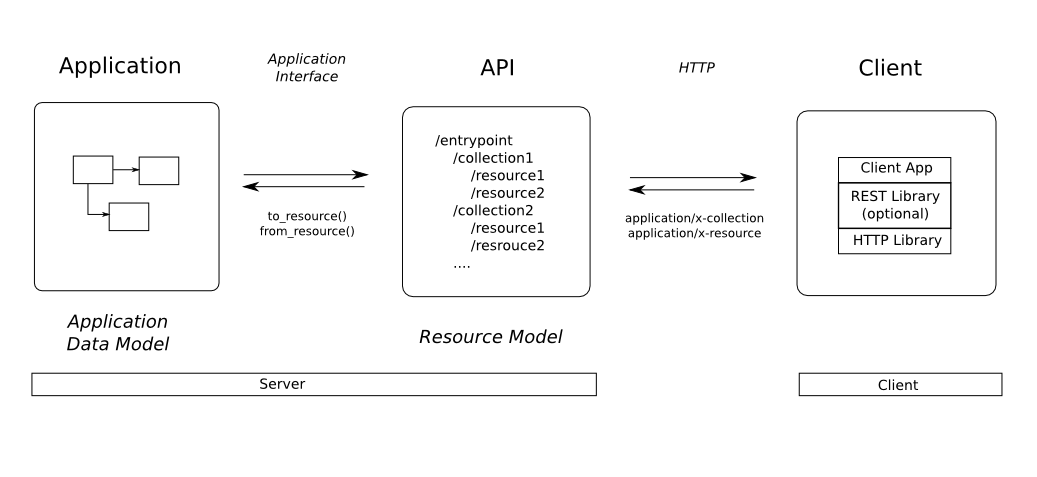
\includegraphics[width=1\textwidth]{rest-scope}
    \caption{Diseño de un API RESTful}
    \label{fig:rest-scope}
\end{figure}

\par \textbf{Servicio web REST}: Es el componente encargado de gestionar las peticiones http a los servicios REST de la Consola de Administración y el API de SidelabCode. Define e implementa la lógica a seguir para la construcción de un proyecto a través de la UI mediante las llamadas ordenadas al API de cada una de las herramientas involucradas en el servicio como componentes de la forja.

\par Los servicios REST ofrecen tres interfaces distintas accesibles a través de http: XML, JSON y HTML para la comunicación la API. Además, hay que desatacar que el servicio web es servido a través del framework \emph{Restlet} a través de Internet de forma continua y remota a cualquier usuario o proceso cliente.

\par Se encarga de la seguridad y validación para las operaciones permitidas o denegadas del usuario de la UI, proporcionando, según su rol, determinados servicios a través de la Consola de Administración, buscar proyectos, crear usuarios, editar proyectos, crear proyectos, etc.

% subsection rest-ws (end)

%%%%%%%%%%%%%%%%%%%%%%%%%%%%%%%%%%%%%%%%%%%%%%%%%%%%%%%%%%%%%%%%%%%%%%%%%%%%%%%%%%%%%%%%%%%%%%%%%%%%%%%%%%
% API
%%%%%%%%%%%%%%%%%%%%%%%%%%%%%%%%%%%%%%%%%%%%%%%%%%%%%%%%%%%%%%%%%%%%%%%%%%%%%%%%%%%%%%%%%%%%%%%%%%%%%%%%%%

\subsection{API}
\label{sub:api}

\par \textbf{API}: La API es el núcleo funcional de SCStack, coordina y realiza las tareas para cada componente de la forja con respecto a los usuarios y proyectos involucrados. Traslada las órdenes ejecutadas en la capa UI a las distintas herramientas para configurar su funcionamiento. Está conectada a todos los servicios que ofrece pivotando a través del directorio LDAP: Control de Versiones, Directorios, Integración Continua, ITS, Revisiones, Gestión de Dependencias, Seguridad y Autenticación que analizaremos extensamente más adelante componente a componente.

% subsection api (end)

% section arquitectura (end)

%%%%%%%%%%%%%%%%%%%%%%%%%%%%%%%%%%%%%%%%%%%%%%%%%%%%%%%%%%%%%%%%%%%%%%%%%%%%%%%%%%%%%%%%%%%%%%%%%%%%%%%%%%
% Aprovisionamiento (Puppet)
%%%%%%%%%%%%%%%%%%%%%%%%%%%%%%%%%%%%%%%%%%%%%%%%%%%%%%%%%%%%%%%%%%%%%%%%%%%%%%%%%%%%%%%%%%%%%%%%%%%%%%%%%%

\section{Aprovisionamiento (Puppet)}
\label{sec:puppet}

\par \emph{Aprovisionamiento}: 'Accción o efecto de aprovisionar', \emph{aprovisionar}: abastecer\footnote{Definición del diccionario de la RAE - \url{http://buscon.rae.es/drae/?type=3&val=aprovisionar&val_aux=&origen=REDRAE}}. Aplicado a la Ingeniería del Software el Aprovisionamiento nos provee de los componentes necesarias para construir una solución.

\par El aprovisionamiento trata de la automatización de tareas para construir el entorno deseado, en este caso la instalación de SidelabCode Stack. La evolución en el modelo de instalación para facilitar la ejecución de módulos, configuración y comunicación entre los distintos componentes.

\par La herramienta empleada para el aprovisionamiento es \textbf{Puppet} de la compañía \emph{PuppetLabs}\footnote{\url{https://puppetlabs.com/}}.

\begin{figure}[H]
    \centering
    
\includegraphics[width=0.3\textwidth]{puppet-labs-logo}
    \caption{Puppet Labs Logo}
    \label{fig:puppet-labs}
\end{figure}

\par \emph{Puppet}: es una herramienta \emph{Software Libre}\footnote{\url{https://puppetlabs.com/puppet/puppet-open-source/}} de aprovisionamiento desarrollada en \emph{Ruby}\footnote{\url{https://github.com/puppetlabs/puppet}}. Gestiona la infraestructura a través de su ciclo de vida, desde el aprovisionamiento y la configuración de parches automatizando la ejecución de órdenes para la instalación y configuración del entorno.

\begin{itemize}
	\item Automatizar tareas repetitivas.
	\item Desplegar rápidamente aplicaciones críticas.
	\item Gestionar proactivamente el cambio.
	\item Escalar de 10 servidores para 1000.
	\item Instalaciones locales o en la nube.
\end{itemize}

\par \emph{Puppet} utiliza un enfoque declarativo, basado en el modelo de automatización:
\begin{itemize}
	\item \emph{Definir} el estado deseado de la configuración de la infraestructura mediante lenguaje de configuración declarativa de Puppet.
	\item \emph{Simular} los cambios de configuración antes de la ejecución.
	\item \emph{Corroborar} el estado final mediante despliegues automáticos comprobando las posibles desviaciones en la configuración.
	\item \emph{Informe} sobre las diferencias entre los estados reales y deseados y cualquier cambio que haya hecho cumplir el estado deseado.
\end{itemize}

\begin{figure}[H]
    \centering
    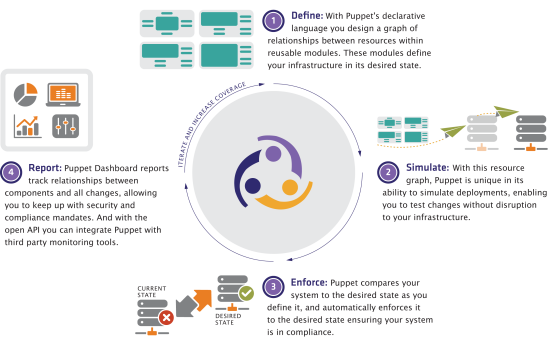
\includegraphics[width=0.7\textwidth]{howpuppetworks}
    \caption{Ciclo de vida de los módulos Puppet}
    \label{fig:howpuppetworks}
\end{figure}

\par El diseño del aprovisionamiento a través de Puppet se basa en módulos. Cada uno de estos módulos se encarga de gestionar la instalación y configuración del componente definido.

\par Que aporta Puppet ? Proporciona un control sobre la instalación de cada herramienta y la configuración asociada por defecto que se define. De esta forma el proceso se instalación se automatiza permitiendo la replicación del mismo, completo o por módulos en diferentes entornos, locales o virtuales. La instalación a partir de módulos ha de definir una cadena de dependencias entre cada uno de ellos de manera que se vayan habilitando funcionalidades e interacciones (Apéndice ~\ref{app:apendice-puppet}).

\par En SidelabCode Stack Puppet es el encargado de gestionar la \emph{instalación y configuración} de cada uno de los componentes mediante módulos Puppet independientes para completar el proceso de instalación (Apéndice ~\ref{app:instalacion-sidelab}) entre 5 y 10 minutos.

%%%%%%%%%%%%%%%%%%%%%%%%%%%%%%%%%%%%%%%%%%%%%%%%%%%%%%%%%%%%%%%%%%%%%%%%%%%%%%%%%%%%%%%%%%%%%%%%%%%%%%%%%%
% Componentes
%%%%%%%%%%%%%%%%%%%%%%%%%%%%%%%%%%%%%%%%%%%%%%%%%%%%%%%%%%%%%%%%%%%%%%%%%%%%%%%%%%%%%%%%%%%%%%%%%%%%%%%%%%

\section{Componentes}
\label{sec:componentes}

\par En este apartado se van a analizar los distintos componentes que integran la Forja SidelabCode Stack y el papel que desempeñan en el funcionamiento del sistema partiendo del esquema en donde se refleja la arquitectura de la Forja SidelabCode ~\ref{fig:scstack-diagram} y la relación que mantienen con las necesidades descritas en el capítulo \nameref{chap:procesos-desarrollo} a la hora de gestionar el proceso \emph{Iterativo e Incremental}.

%%%%%%%%%%%%%%%%%%%%%%%%%%%%%%%%%%%%%%%%%%%%%%%%%%%%%%%%%%%%%%%%%%%%%%%%%%%%%%%%%%%%%%%%%%%%%%%%%%%%%%%%%%
% OpenLDAP
%%%%%%%%%%%%%%%%%%%%%%%%%%%%%%%%%%%%%%%%%%%%%%%%%%%%%%%%%%%%%%%%%%%%%%%%%%%%%%%%%%%%%%%%%%%%%%%%%%%%%%%%%%

\subsection{Usuarios, roles y grupos}
\label{sub:usuarios-roles-grupos}

\par Gestión de usuarios, roles, grupos y proyectos a través de \emph{OpenLDAP}\footnote{OpenLDAP - \url{http://www.openldap.org/}}.

\begin{figure}[H]
    \centering
    
\includegraphics[width=0.3\textwidth]{OpenLDAP-logo}
    \caption{OpenLDAP logo}
    \label{fig:openldap-logo}
\end{figure}

\par SCStack utiliza la tecnología de directorios \emph{LDAP} como sistema de autenticación y de información centralizado de la Forja Software. En dicho servidor de directorios se almacena información relativa a todos los usuarios, proyectos software y repositorios de la Forja. Esta tecnología, además, cuenta con la ventaja de que la mayoría de aplicaciones web con sistemas de autenticación ofrecen interfaces que garantizan una completa integración con directorios LDAP, este es el caso de Redmine, Drupal, Wordpress y el propio servidor web Apache. La implementación de este protocolo en la Forja Sidelab se lleva a cabo mediante un servidor de directorios muy estable y de libre distribución que es OpenLDAP.

\subsection{API OpenLDAP}
\label{sub:api-openldap}

\par Debido a que el directorio LDAP es la estructura de información centralizada de la Forja, cualquier tipo de acción que se quiera realizar sobre el sistema requerirá el acceso por parte de la API a este servicio de directorios, bien para la recuperación de datos en las consultas o para la manipulación de registros a la hora de crear, editar o borrar usuarios o proyectos.

\par Todas las acciones de la Consola de Administración pasan a través de la API que comunica con OpenLDAP dando acceso y generando las distintas autenticaciones en cada una de las herramientas interconectadas basándose en los registros de OpenLDAP como generador y autenticador de credenciales.

% subsection api-openldap (end)

% subsection usuarios-roles-grupos (end)

%%%%%%%%%%%%%%%%%%%%%%%%%%%%%%%%%%%%%%%%%%%%%%%%%%%%%%%%%%%%%%%%%%%%%%%%%%%%%%%%%%%%%%%%%%%%%%%%%%%%%%%%%%
% Gestión de Requisitos - Redmine
%%%%%%%%%%%%%%%%%%%%%%%%%%%%%%%%%%%%%%%%%%%%%%%%%%%%%%%%%%%%%%%%%%%%%%%%%%%%%%%%%%%%%%%%%%%%%%%%%%%%%%%%%%

\subsection{Gestión de Requisitos ITS}
\label{sub:its}

\par La gestión de requisitos en SidelabCode Stack se lleva a cabo a través del Issue Tracking System \emph{Redmine}\footnote{Redmine - \url{http://www.redmine.org/}}.

\begin{figure}[H]
    \centering
    
\includegraphics[width=0.3\textwidth]{redmine}
    \caption{Redmine logo}
    \label{fig:redmine-logo}
\end{figure}

\par Este apartado es el más cuidado e importante en el conjunto de SCStack ya que se trata de la herramienta encargada de centralizar la gestión de \emph{Lista de Control del Proyecto} por cada Iteración. El ITS Redmine es una aplicación web de gestión de proyectos Software multiplataforma desarrollada en \emph{Ruby} a través de \emph{Ruby on Rails}. Por supuesto se trata de una herramienta FLOSS.

\par Redmine proporciona la gestión de tareas (de cualquier tipo; \emph{features, bugs, parches\ldots}) para cada uno de los proyectos creados. Dentro de SCStack se encuentra enlazado a la configuración de usuarios a través de OpenLDAP para la validación y cuenta con una base de datos propia \emph{MySQL}. Un apartado importante ya que esto permite gestionar las migraciones de Redmine de manera rápida, eficiente y fluida de una versión a otra o incluir la información de otro Redmine\footnote{Upgrading Redmine - \url{http://www.redmine.org/projects/redmine/wiki/RedmineUpgrade}} en una nueva instalación de la Forja, únicamente haciendo un backup de la base de datos y algunos directorios clave. Incluso la migración a Redmine desde otros gestores de tareas\footnote{Migrate to Redmine - \url{http://www.redmine.org/projects/redmine/wiki/RedmineMigrate}}.

\par Proporciona una interfaz adaptada para cada proyecto de la forja asociado a un repositorio de código fuente con un visor integrado. Se visualizan los cambios entre distintas versiones del código y comparaciones entre distintas ramas de desarrollo para seguir la evolución del proyecto.

\begin{figure}[H]
    \centering
    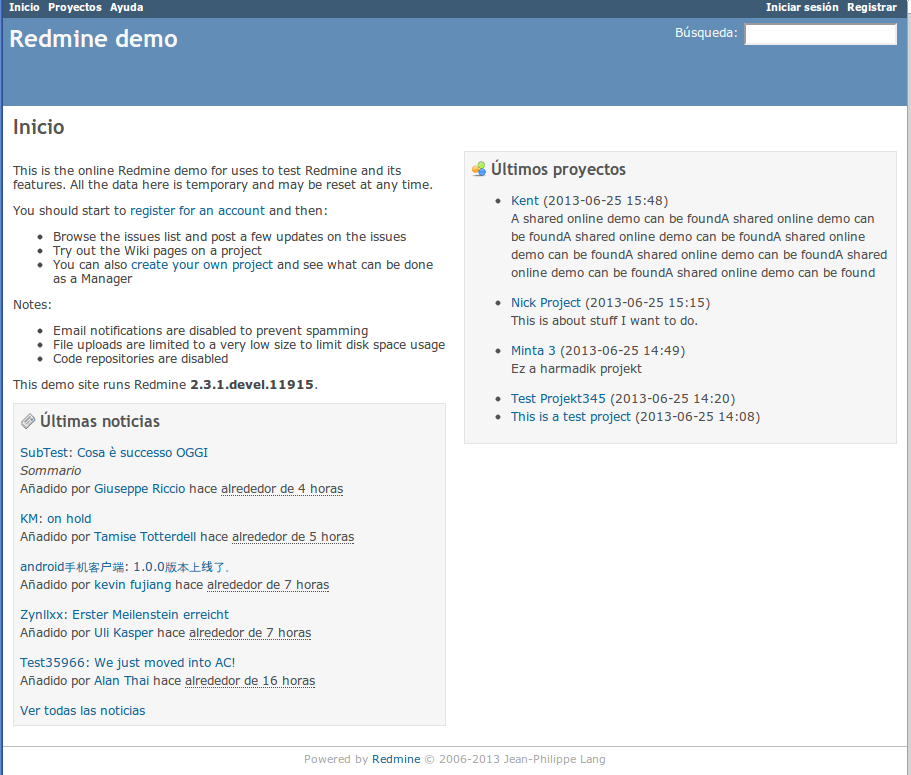
\includegraphics[width=0.7\textwidth]{redmine-demo-landing-page}
    \caption{Redmine página de bienvenida}
    \label{fig:redmine-demo-landing-page}
\end{figure}

\par Dentro del proceso Iterativo e Incremental como herramientas nos proporciona informes de seguimiento de actividad dinámicos (\emph{día, persona, proyecto\ldots}), un \emph{Wiki} para la documentación y una página de noticias.

\par Es la interfaz web de entrada al proyecto para los desarrolladores, por ello es la parte más importante y en donde se centran gran parte de los esfuerzos para la fluidez y la importancia que tiene la misma.

\par Por otra parte Redmine proporciona una API Rest para facilitar la interoperabilidad entre los distintos componentes. Esta API se maneja a través de la capa de negocio de la Consola de Administración de SCStack para así a través del API se registren en Redmine los usuarios, proyectos y grupos con sus respectivos permisos partiendo de los valores introducidos a través de la Consola de Administración. De esta forma, Redmine pasa a gestionar a través de su BBDD MySQL los usuarios y proyectos después que se hayan autenticado a través de OpenLDAP para así cargar la configuración obtenida de su BBDD.

\par Las operaciones de gestión administrativa en Redmine permanecen desactivadas, de modo que ningún administrador de proyectos puede añadir ni borrar miembros de sus proyectos, tampoco pueden crearse ni borrarse usuarios o proyectos, etc. \emph{Obligando} así que todas las operaciones de gestión de la Forja se lleven a cabo desde el Software diseñado específicamente para ello, la Consola de Administración, garantizando así la consistencia.

\subsection{Plugins}
\label{sub:redmine-plugins}

\par A la hora de aplicar el desarrollo Iterativo e Incremental se intenta incrementar la eficacia, la visibilidad, la rapidez y la comprensión del proceso de desarrollo. Por eso se han utilizado distintos plugins para Redmine que ayudan a la comprensión y agilizan el proceso Iterativo e Incremental para los usuarios (desarrolladores, gestores, etc\ldots) a través del plugin FLOSS \emph{Backlogs}\footnote{Redmine Backlogs - \url{http://www.redminebacklogs.net/}}.

\par \emph{Backlogs} aporta una gestión visual en modo tablón de las Iteraciones activas en el proceso. Gestiona 'manualmente' a través de \emph{Drag and Drop} la organización de las tareas del proyecto y agiliza la comprensión del estado de la iteración, proyecto, desarrollo en sí, en un sólo vistazo ~\ref{fig:backlogs-plugin}.

\begin{figure}[H]
    \centering
    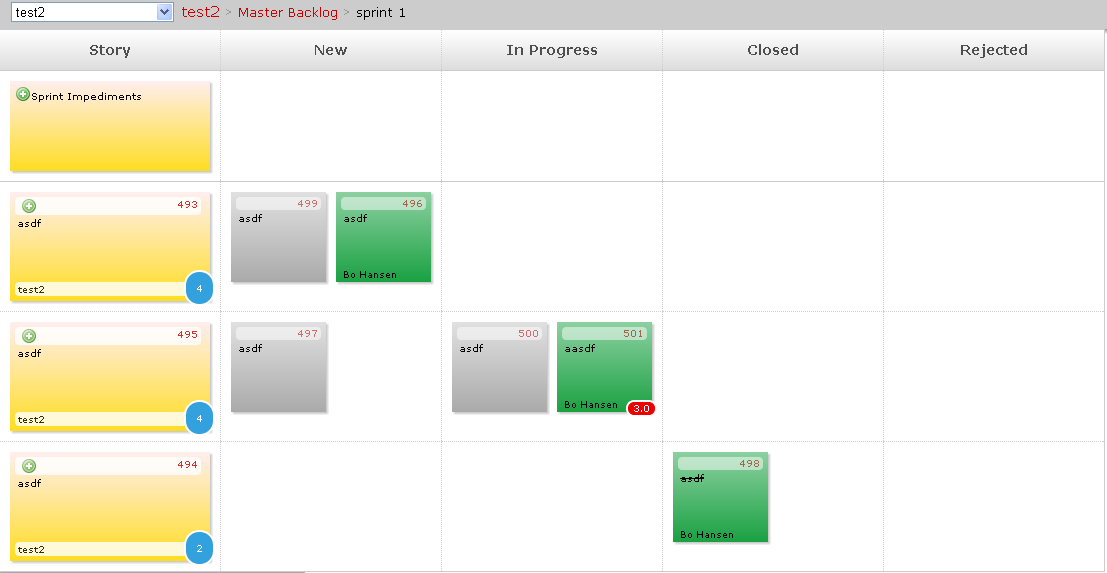
\includegraphics[width=0.7\textwidth]{backlogs-plugin}
    \caption{Redmine Backlogs plugin: tareas Redmine agrupadas por estados dentro de una historia de usuario.}
    \label{fig:backlogs-plugin}
\end{figure}

\par Otro apartado importante en el desarrollo Iterativo e Incremental es la gestión de la documentación, en este caso Redmine nos proporciona una Wiki por cada proyecto. Una Wiki es una herramienta para la documentación colaborativa que mantiene su histórico de cambios (asociados a usuario y tiempo) y que mediante el lenguaje de marcado wiki desde el cual se exportan a distintos formatos como: \emph{html, pdf, etc}, a un coste de recursos bajo ya que se trata de texto plano. El caso más famoso del uso de Wikis como documentación colaborativa es la \emph{Wikipedia}\footnote{Wikipedia - \url{http://www.wikipedia.org}}.

% subsection redmine-plugins (end)

% subsection its (end)

%%%%%%%%%%%%%%%%%%%%%%%%%%%%%%%%%%%%%%%%%%%%%%%%%%%%%%%%%%%%%%%%%%%%%%%%%%%%%%%%%%%%%%%%%%%%%%%%%%%%%%%%%%
% Repositorios de Código
%%%%%%%%%%%%%%%%%%%%%%%%%%%%%%%%%%%%%%%%%%%%%%%%%%%%%%%%%%%%%%%%%%%%%%%%%%%%%%%%%%%%%%%%%%%%%%%%%%%%%%%%%%

\subsection{Repositorios de Código}
\label{sub:repositorios}

\par Los repositorios de código (VCS) son los encargados de gestionar el ciclo de vida del código fuente como hemos visto en el apartado de Código versionado~\ref{sec:codigo-versionado} y existen dos tipos: centralizados y distribuidos. Para el proceso de desarrollo Iterativo e Incremental hemos seleccionado el repositorio distribuido \emph{Git}\footnote{Git - \url{http://git-scm.com/}}.

\begin{figure}[H]
    \centering
    
\includegraphics[width=0.3\textwidth]{git-logo}
    \caption{Git SCM Logo}
    \label{fig:git-scm-logo}
\end{figure}

\par Atendiendo a los requerimientos del proceso:

\begin{quote}
    \emph{El desarrollo de la solución se adapta al uso del Repositorio distribuido, ya que éste aporta una flexibilidad para la gestión de bifurcaciones del código que en un repositorio centralizado no tenemos fácilmente}
\end{quote}

\par En el proceso Iterativo e Incremental abundan las ramificaciones del código en el repositorio debido a ello se opta por la elección del repositorio distribuido Git en pro del repositorio centralizado SVN, que también se incluye en la Forja SCStack. Las ramificaciones, la cantidad de fusiones entre ramas~\cite{featurebranch}, entornos de desarrollo sumando la facilidad, agilidad y el bajo coste en Git nos proporcionan la herramienta adecuada para la gestión del código fuente en SCStack.

\par En el repositorio Git no se guardan diferencias se guardan snapshots en comparación con Subversion.

\begin{figure}[H]
    \centering
    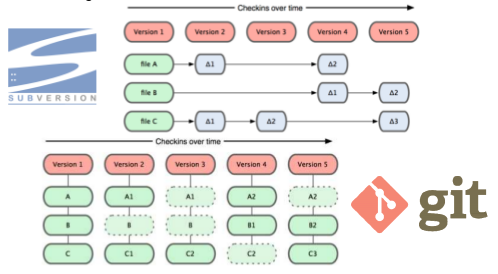
\includegraphics[width=0.7\textwidth]{svn-git-comparison}
    \caption{Comparación de incrementos entre SVN (completo) y Git (incrementos en archivos)}
    \label{fig:svn-git-comparison}
\end{figure}

\begin{quotation}
    \emph{For example the Mozilla repository is reported to be almost 12 Gb when stored in SVN using the fsfs backend. Previously, the fsfs backend also required over 240,000 files in one directory to record all 240,000 commits made over the 10 year project history. This was fixed in SVN 1.5, where every 1000 revisions are placed in a separate directory. The exact same history is stored in Git by only two files totaling just over 420 Mb. This means that SVN requires 30x the disk space to store the same history}\footnote{Git Svn Comparison Smaller Space Requirements - \url{https://git.wiki.kernel.org/index.php/GitSvnComparison\#Smaller\_Space\_Requirements}}
\end{quotation}

\par Asociada a cada Iteración se ha de gestionar la viabilidad de una rama del repositorio. En esta rama se trabaja con respecto a las tareas a desarrollar para la iteración. Se hacen las pruebas necesarias para cada desarrollo para después integrar la solución en la rama principal y así crear una nueva versión del proyecto. 

\par La ramificación del desarrollo permite gestionar por iteraciones incrementales aisladas en una nueva rama, de esta forma, el contenido de la rama principal es fiable, ya que para añadir contenido a la rama ha tenido que pasar una iteración nueva y el proceso de desarrollo que conlleva; planificación, test, implementación e integración. El resultado está altamente controlado y distribuido en base a módulos para poder acotar posibles errores posteriores o revertir cambios a través de un proceso minuciosamente controlado.

\subsubsection{Integridad}
\label{subs:git-integridad}

\par Los commits se identifican por un \texttt{hash sha1}

\begin{itemize}
    \item \texttt{Svn}: \emph{rev 33}
    \item \texttt{Git}: \emph{d025a7b3217f05110ebbf48065b8d02a0ad22ae3}
\end{itemize}

\par O más amigablemente: \emph{d025a7b}

\par Los ficheros también se identifican por su sha1 de esta forma si un fichero se corrompe durante la transmisión por la red se detecta inmediatamente

\subsubsection{Los 3 estados}
\label{subs:git-3-estados}

\par Los ficheros en Git pueden estar en tres estados:

\begin{itemize}
    \item \texttt{Modificado}: el fichero ha cambiado desde el último checkout
    \item \texttt{Staged}: un fichero modificado ha sido marcado para ser añadido en el próximo commit
    \item \texttt{Committed}: el fichero se encuentra en la base de datos de git
\end{itemize}

\par Hay un 4º estado: \textbf{untracked}.

\subsubsection{Las 3 áreas de un proyecto git}
\label{subs:git-3-areas}

\begin{enumerate}
    \item El directorio git (git directory):
        \begin{itemize}
            \item Contiene los metadatos y la base de datos de git
            \item Es lo que se copia cuando se clona un repositorio
            \item Normalmente es una carpeta .git en algún directorio
        \end{itemize}
    \item La carpeta de trabajo (working directory):
        \begin{itemize}
            \item Es un checkout de una versión específica del proyecto
            \item Se extrae del directorio git
            \item Es el espacio donde modificamos los ficheros
        \end{itemize}
    \item Staging area:
        \begin{itemize}
            \item Fichero en el directorio git que indica qué cambios van en el próximo commit
        \end{itemize}
\end{enumerate}

\begin{figure}[H]
    \centering
    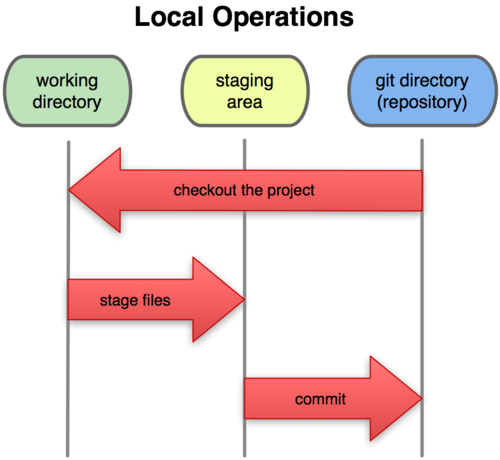
\includegraphics[width=0.7\textwidth]{git-3-areas}
    \caption{Tres áreas en Git}
    \label{fig:git-3-areas}
\end{figure}

\subsubsection{La identidad}
\label{subs:git-identidad}

\par Git necesita conocer algunos datos del desarrollador (aparecen en los commits para identificar al autor)

\begin{itemize}
    \item Nombre
    \item Email
\end{itemize}

\par Si no están correctamente configurados pueden aparecer varios problemas:

\begin{itemize}
    \item Los commits \textbf{fallan} porque el usuario no está autorizado
    \item Commits del mismo usuario \emph{'físico'} \textbf{no son considerados como del mismo usuario} porque el nombre \emph{'lógico'} cambia.
\end{itemize}

\par Por lo que se ha de tener muy en cuenta este apartado y configurar correctamente en el archivo.

% subsection repositorios (end)

\subsection{Revisión de Código}
\label{sub:gerrit}

\par La gestión del repositorio Git está orientada a través de la herramienta \emph{Gerrit}\footnote{\url{http://code.google.com/p/gerrit/}}.

\begin{figure}[H]
    \centering
    
\includegraphics[width=0.3\textwidth]{gerrit-diffy}
    \caption{Gerrit Kunfu Review Cuckoo}
    \label{fig:gerrit-logo}
\end{figure}

\par Gerrit es una herramienta de revisión de código basada en web. Facilita el control online de las revisiones de código para los proyectos a través de la herramienta Git.

\par Gestiona la autenticación y la gestión de permisos, roles y grupos para cada uno de los repositorios existentes a través de una interfaz ligera. Un punto a destacar es la orientación hacia un repositorio centralizado de Git, es decir, el control de código se centraliza en un repositorio para la integración dependiente de los repositorios de los desarrolladores\footnote{Git Flujo de trabajo centralizado - \url{http://git-scm.com/book/es/Git-en-entornos-distribuidos-Flujos-de-trabajo-distribuidos\#Flujo-de-trabajo-centralizado}}.

\begin{figure}[H]
    \centering
    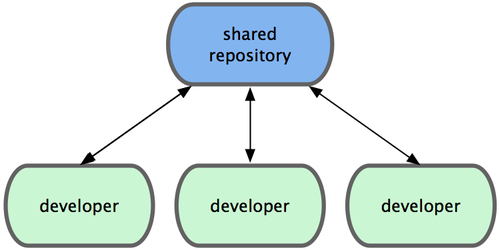
\includegraphics[width=0.7\textwidth]{git-centralizado}
    \caption{Git: Flujo de trabajo centralizado}
    \label{fig:git-centralizado}
\end{figure}

\par Centralizar la rama principal del proyecto en el repositorio descentralizado casa perfectamente con el proceso Iterativo e Incremental ya que a cada iteración cerrada añadimos los cambios a la rama estable del proyecto desarrollado centralizando el código a empaquetar para convertir en la solución final, incremento a incremento.

\par La configuración viene a través del API de SCStack y una consola interactiva SSH\footnote{Gerrit Command Line Tools - \url{http://gerrit.googlecode.com/svn/documentation/2.0.34/cmd-index.html}} que proporciona Gerrit. En SCStack esta función recae sobre los valores obtenidos del servidor \emph{OpenLDAP} a partir de los datos introducidos en la Consola de Administración a la hora de gestionar la creación de un proyecto y el grupo de usuarios asociados al proyecto siguiendo el flujo de datos centralizado a través de la API Rest central. La creación del proyecto, la gestión de usuarios y permisos sobre el repositorio Git creado.

\par Este procedimiento se encapsula a través del envío de órdenes a la consola a través del API habiendo configurado la autenticación a través de un conjunto de clave SSH en la instalación de SCStack.

% subsection gerrit (end)

%%%%%%%%%%%%%%%%%%%%%%%%%%%%%%%%%%%%%%%%%%%%%%%%%%%%%%%%%%%%%%%%%%%%%%%%%%%%%%%%%%%%%%%%%%%%%%%%%%%%%%%%%%
% Integración Continua
%%%%%%%%%%%%%%%%%%%%%%%%%%%%%%%%%%%%%%%%%%%%%%%%%%%%%%%%%%%%%%%%%%%%%%%%%%%%%%%%%%%%%%%%%%%%%%%%%%%%%%%%%%

\subsection{Integración Continua}
\label{sub:ci-jenkins}

\par  La integración continua dentro del proceso de desarrollo Iterativo e Incremental es la encargada de agilizar la comunicación entre los distintos actores involucrados. Evalúa la evolución de la solución y provee una respuesta firme y profesional para afianzar los resultados de cada incremento.

\begin{figure}[H]
    \centering
    
\includegraphics[width=0.3\textwidth]{jenkins}
    \caption{Jenkins CI Logo}
    \label{fig:jenkins-logo}
\end{figure}


\par En este aspecto, la herramienta que SCStack necesita es un gestor de integración continua como \emph{Jenkins-CI}\footnote{Jenkins-CI - \url{http://jenkins-ci.org}}:

\begin{quote}
    \emph{In a nutshell Jenkins CI is the leading open-source continuous integration server. Built with Java, it provides over 400 plugins to support building and testing virtually any project.}
\end{quote}

\par Jenkins-CI\footnote{Meet Jenkins-CI - \url{https://wiki.jenkins-ci.org/display/JENKINS/Meet+Jenkins}} proporciona la integración de la integración continua (valga la redundancia) en el proceso de desarrollo de software de una forma modular e interoperable. No se trata de un servidor intrusivo ni para el proceso de desarrollo ni para el desarrollador en si.

\par En este aspecto SCStack incluye el módulo de Jenkins-CI en la instalación para facilitar el trabajo de las pruebas, integración y generación de versiones mediante la virtualización de escenarios más cercanos al sistema de producción. Des esta forma se perfila mejor el rendimiento, la replicación de errores y el control de la evolución del código fuente. Dentro del desarrollo, el código fuente es el centro de la calidad y debido a esta afirmación, se necesita un servidor de CI adaptado al proceso de desarrollo.

\begin{itemize}
	\item Tags.
	\item Construir las versiones vivas.
	\item Branches de releases.
	\item Desplegar una versión específica con un clic.
\end{itemize}

\par Jenkins-CI se instala integrado en el marco de trabajo SCStack interoperando entre el repositorio de código fuente Git, la herramienta de gestión Gerrit y el despliegue de los tests en servidores como Apache o Tomcat dependiendo del producto final (esto no tiene nada que ver con el desarrollo, sería un requisito del proyecto). Jenkins-CI mantiene diferentes versiones vivas a la vez en el repositorio del proyecto para cumplir con los objetivos:

\begin{itemize}
	\item Asegurar la calidad.
	\item Hacer el despliegue ágil.
	\item Minimizar el riesgo.
\end{itemize}

\par Jenkins-CI trabaja en base a \emph{Jobs}. Un Job en Jenkins-CI describe el proceso de integración, pruebas o despliegue que va a ejecutarse cuando se cumpla un requisito definido o manualmente. La integración de las distintas ramas de desarrollo en cada iteración en el ciclo de vida~\ref{fig:simple-lifecycle} las gestiona Jenkins-CI a través de los Jobs definidos:

\begin{itemize}
	\item Jobs de \emph{integración}.
	    \begin{itemize}
        	\item Descargan el código del repositorio Git.
        	\item Construyen.
        	\item Pasan tests.
        	\item Despliegan la versión construida en "local".
        \end{itemize}
	\item Jobs de \emph{release}.
	    \begin{itemize}
        	\item Realizan los pasos anteriores y además.
        	\item Tag si los tests pasaron.
        	\item Push del tag al repositorio remoto.
        \end{itemize}
	\item Jobs de \emph{despliegue}.
	    \begin{itemize}
        	\item Descargan el binario del repositorio de binarios
        	\item Desplegar en un servidor de aplicaciones.
        \end{itemize}
\end{itemize}

\begin{figure}[H]
    \centering
    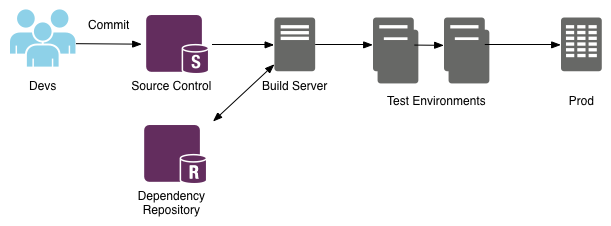
\includegraphics[width=0.7\textwidth]{simple-lifecycle}
    \caption{Ciclo de vida Jenkins CI}
    \label{fig:simple-lifecycle}
\end{figure}

\par Dentro de la forja SCStack se configura el uso de Jenkins-CI a partir de usuarios dedicados a la gestión de jobs. Se plantean tres opciones:

\begin{itemize}
	\item \textbf{Opción I}: Un usuario \emph{jenkinsci} con acceso de \emph{lectura/escritura} a \emph{todos} los repositorios.
        \begin{itemize}

        	\item \emph{Pros}; Simplicidad: sólo hay que gestionar un usuario. Una \emph{única} clave ssh \emph{/home/tomcat/.ssh/id\_rsa.pub}.
        	\item \emph{Contras}; Un usuario para dominarlos a todos. Cualquier error en un job para el proyecto \emph{X} puede afectar a los repositorios del proyecto \emph{Y}.
        \end{itemize}

	\item \textbf{Opción II}: Un usuario @jenkinsci@ con acceso de \emph{lectura/escritura} a todos los repositorios y  otro \emph{jenkinsci\_read} con acceso sólo de lectura	
        \begin{itemize}
        	\item \emph{Pros}; Sólo hay que gestionar \emph{dos usuarios}: basta con asociarlos a \emph{todos} los proyectos.
        	\item \emph{Contras}; Seguimos teniendo un usuario para dominarlos a todo: jenkinsci. Cualquier error en un job para el proyecto \emph{X} puede afectar a los repositorios del proyecto \emph{Y}. Hay que gestionar dos claves ssh. No es trivial.
        \end{itemize}

	\item \textbf{Opción III}: Un \emph{usuario por proyecto} para integración continua.
        \begin{itemize}
        	\item \emph{Pros}; El usuario de ci de un proyecto no tiene acceso a los repositorios de otro proyecto.
        	\item \emph{Contras}; Hay que gestionar múltiples \emph{claves ssh}.
        \end{itemize}

\end{itemize}

\par Se decide utilizar un usuario por proyecto definida en la \textbf{tercera opción}, después de haber evaluado las distintas opciones.
 
\par La gestión de los usuarios se gestiona a través de la consola de administración de SCStack. De esta manera la herramienta nos aporta una vía única de entrada dotando de la funcionalidad específica para distintos estados del proceso de desarrollo nada intrusivos en el desarrollo del proyecto. Separando a través del API de SCStack la gestión y partiendo de los roles/usuarios/grupos definidos como base en OpenLDAP.

\par El repositorio remoto debería contener versiones más o menos estables y distinguidas para el desarrollo por ramas establecido el proceso:

\begin{itemize}
	\item \textbf{Develop}: Pueden fallar algunos tests, no es problema.

	\item \textbf{Release-X}: Los tests deberían pasar, eventualmente se podrían desactivar.
	
	\item \textbf{Nightly builds}: Construcciones que comprueban la \emph{'salud'} del proyecto. Se hacen sobre los branches \emph{development} y \emph{release-X} (siendo X la versión más reciente).

    \begin{itemize}
	    \item Se ejecutan los tests.
	    \item Se despliegan dos versiones por cada rama: \texttt{Limpia}: una bbdd nueva y \texttt{Migración}: con actualización de bbdd ya existente sobre la bbdd que ya hubiera para ese despliegue.
    \end{itemize}

	\item \textbf{Preproducción}: Las versiones que van a preproducción son aquellas de las que se ha hecho \texttt{tag}: 
	\begin{itemize}
	    \item Pasan los tests.
	    \item El entorno de pre puede estar en \emph{local} o en \emph{Remoto}.
	    \item Se despliegan dos versiones: \texttt{Limpia} y \texttt{Migración}.
    \end{itemize}

	\item \textbf{Producción}: Las versiones que van a producción son aquellas de las que se ha hecho \texttt{tag}.
	\begin{itemize}
	    \item Pasan los tests.
	    \item El despliegue se realiza en \emph{Remoto}.
	    \item Se despliegan dos versiones: \texttt{Limpia} y \texttt{Migración}.
    \end{itemize}

\end{itemize}

\begin{figure}[H]
    \centering
    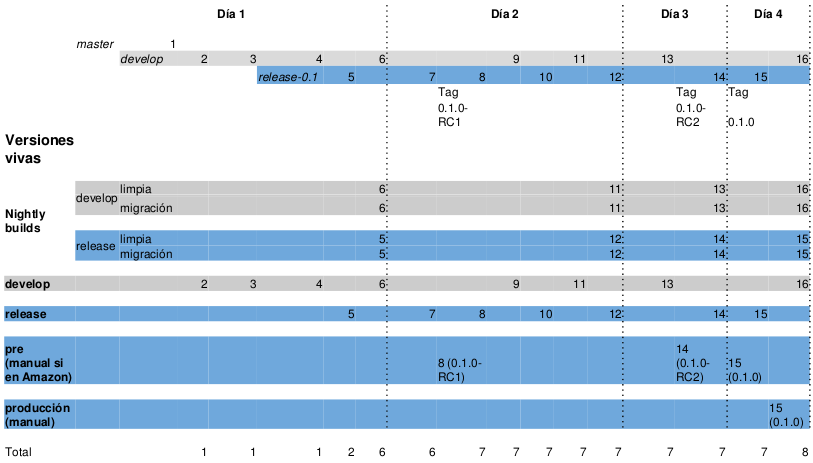
\includegraphics[width=0.7\textwidth]{diagrama-integracion-continua}
    \caption{Integración Continua de versiones a partir de distintas ramas}
    \label{fig:diagrama-integracion-continua}
\end{figure}

% subsection ci-jenkins (end)

%%%%%%%%%%%%%%%%%%%%%%%%%%%%%%%%%%%%%%%%%%%%%%%%%%%%%%%%%%%%%%%%%%%%%%%%%%%%%%%%%%%%%%%%%%%%%%%%%%%%%%%%%%
% Gestión de distribuciones y dependencias
%%%%%%%%%%%%%%%%%%%%%%%%%%%%%%%%%%%%%%%%%%%%%%%%%%%%%%%%%%%%%%%%%%%%%%%%%%%%%%%%%%%%%%%%%%%%%%%%%%%%%%%%%%

\subsection{Gestión de distribuciones y dependencias}
\label{sub:distribuciones-dependencias}

\par Gestión de recursos compartidos, comunicación segura a través de \emph{OpenSSH} y gestión de dependencias y distribuciones a través de \emph{Archiva} como repositorio \emph{Maven}.

\subsubsection{OpenSSH}
\label{ssub:openssh}

\par \emph{OpenSSH}\footnote{\url{http://www.openssh.org/}} es un conjunto de aplicaciones de libre distribución que permiten realizar comunicaciones cifradas a través de la red usando el protocolo SSH.

\begin{figure}[H]
    \centering
    
\includegraphics[width=0.3\textwidth]{openssh_logo}
    \caption{OpenSSH logo}
    \label{fig:openssh_logo}
\end{figure}

\par La función fundamental que brinda este protocolo a la Forja Software consiste en garantizar que los usuarios de los distintos proyectos puedan acceder, por ejemplo a través de SFTP\footnote{\url{http://en.wikipedia.org/wiki/SFTP}} o Secure Shell \emph{SSH}\footnote{\url{http://en.wikipedia.org/wiki/Secure\_Shell}}, a las carpetas privadas y públicas de los proyectos en los cuales participan, a través de una conexión cifrada, y gestionar sus ficheros de una forma sencilla, ágil y segura.

% subsubsection openssh (end)

\subsubsection{Archiva}
\label{ssub:archiva}

\par \emph{Archiva}\footnote{\url{http://archiva.apache.org/index.cgi}} es una aplicación FLOSS para la gestión de repositorios de artefactos de construcción, desarrollado por \emph{Apache Software Foundation}. Este el compañero perfecto para herramientas de construcción como Maven.

\begin{figure}[H]
    \centering
    
\includegraphics[width=0.3\textwidth]{apache-archiva-logo}
    \caption{Apache Archiva logo}
    \label{fi:apache-archiva}
\end{figure}

\par Entre las funcionalidades que podemos destacar de esta herramienta están, el proxy para repositorio remoto (reduce el tráfico de red en equipos de trabajo), la gestión del control de acceso a los repositorios definidos, la construcción de artefactos de almacenamiento y, la gestión y mantenimiento de repositorios Maven facilitando la indexación, búsquedas, informes, estadísticas.

\par Posee una interfaz web sencilla de configurar en la que publica el contenido del repositorio Maven accesible a los usuarios autenticados. Además de el acceso al repositorio Maven habiendo configurado en los proyectos de desarrollo la url en la que está publicado:

\lstset{style=xmlbasico}
\begin{lstlisting}[frame=trbl]
<project>
  <!-- omitted xml -->
  <distributionManagement>
    <repository>
      <id>archiva.internal</id>
      <name>Internal Release Repository</name>
      <url>http://reposerver.mycompany.com:8080/archiva/repository/internal/</url>
    </repository>
    <snapshotRepository>
      <id>archiva.snapshots</id>
      <name>Internal Snapshot Repository</name>
      <url>http://reposerver.mycompany.com:8080/archiva/repository/snapshots/</url>
    </snapshotRepository>
  </distributionManagement>
  <!-- omitted xml -->
</project>
\end{lstlisting}

\par El uso de Archiva como gestor de dependencias Maven puede ser público y/o privado dependiendo del repositorio que se cree. De esta forma los equipos de desarrolladores automatizan y centralizan las descargas de las dependencias (librerías) a través de Archiva dentro de la red local, disminuyendo el tráfico de red y agilizando la puesta en marcha de proyectos y los jobs de CI, reduciendo el consumo.

% subsubsection archiva (end)

% subsection distribuciones-dependencias (end)

% subsection componentes (end)

%%%%%%%%%%%%%%%%%%%%%%%%%%%%%%%%%%%%%%%%%%%%%%%%%%%%%%%%%%%%%%%%%%%%%%%%%%%%%%%%%%%%%%%%%%%%%%%%%%%%%%%%%%
% Desarrollo Eclipse y Maven
%%%%%%%%%%%%%%%%%%%%%%%%%%%%%%%%%%%%%%%%%%%%%%%%%%%%%%%%%%%%%%%%%%%%%%%%%%%%%%%%%%%%%%%%%%%%%%%%%%%%%%%%%%

\subsection{Desarrollador: Eclipse y Maven}
\label{sub:eclipse-mvn-tdd}

\par El entorno de desarrollo para el desarrollador en el que se integra el proceso Iterativo e Incremental consta de dos herramientas y un concepto.

\par El IDE \emph{Integrated Development Environment} a utilizar es Eclipse, concretamente la distribución del framework Spring \emph{Eclipse STS}\footnote{Eclipse STS - \url{http://www.springsource.org/sts}}. 

\begin{figure}[H]
    \centering
    
\includegraphics[width=0.3\textwidth]{STS}
    \caption{Spring Tool Suite logo}
    \label{fig:sts}
\end{figure}

\par STS otorga y proporciona un conjunto de herramientas preparadas para trabajar con los componentes de STStack: Redmine, Git, Gerrit, Jenkins, Apache, OpenLDAP, Maven. Se basa en unan distribución de Eclipse orientada al desarrollo para trabajar con diferentes componentes externos facilitando la puesta a punto para empezar a desarrollar.

\par Esta distribución incluye la gestión de un proyecto a través \emph{Maven}\footnote{Apache Maven - \url{http://maven.apache.org/}}. Maven es un Software de gestión de proyectos basado en la definición del proyecto POM (Project Object Model). Es el encargado de compilar, ejecutar test, desplegar, gestionar las dependencias (locales y remotas) y generar distribuciones a partir de una configuración definida.

\begin{figure}[H]
    \centering
    
\includegraphics[width=0.3\textwidth]{maven}
    \caption{Maven logo}
    \label{fig:maven-logo}
\end{figure}

\par Esta herramienta se integra en el ciclo de vida del Software para automatizar los procesos tediosos manuales, proveer una estructura básica inicial a los proyectos (iteración 0) para ir incrementando iteración tras iteración a través de los arquetipos.

\par Incorpora componentes en la instalación por defecto para facilitar el trabajo del desarrollador con la forja SCSTack:

\begin{itemize}
	\item \emph{Egit} - Plugin de Eclipse para trabajar con repositorios Git - \url{http://www.eclipse.org/egit/}.
	\item \emph{Mylyn} - Plugin para gestionar las tareas del ITS, en este caso Redmine, a través de la interfaz de Eclipse. Automatizando las pruebas, grabando sesiones de trabajo e incluso compartirlas para poder reproducir un procedimiento en otro sistema - \url{http://www.eclipse.org/mylyn/}
	\item \emph{Maven} - Plugin \emph{2eclipse} para la gestión de proyectos Maven a través de su ciclo de vida. Ayuda a facilitar la configuración de los builds a través de los pom de Maven. Genera esqueletos de proyectos a través de los arquetipos de una forma intuitiva - \url{http://www.sonatype.org/m2eclipse}
\end{itemize}

\par A través de Maven y Eclipse se definen las líneas del desarrollo de cada iteración facilitando el diseño TDD~\ref{sub:tdd} a través de una sencilla configuración. El esqueleto de los proyectos Maven proporciona unas sencillas guías estándar para el desarrollo de proyectos de Software. Esta agrupación de funcionalidades se reutiliza en Jenkins-CI a través de los \emph{jobs} de Maven para así poder replicar cualquier entorno durante la integración continua partiendo de una base robusta.

% subsection eclipse-mvn-tdd (end)

%%%%%%%%%%%%%%%%%%%%%%%%%%%%%%%%%%%%%%%%%%%%%%%%%%%%%%%%%%%%%%%%%%%%%%%%%%%%%%%%%%%%%%%%%%%%%%%%%%%%%%%%%%
% Pruebas y Validación
%%%%%%%%%%%%%%%%%%%%%%%%%%%%%%%%%%%%%%%%%%%%%%%%%%%%%%%%%%%%%%%%%%%%%%%%%%%%%%%%%%%%%%%%%%%%%%%%%%%%%%%%%%

\section{Pruebas y Validación}
\label{sec:pruebas-validacion}

\par Todo proyecto de software necesita ser probado para comprobar que funcione correctamente si existen fallos para así poder atajarlos sin que las sorpresas aparezcan.

\par El lenguaje utilizado para el desarrollo del API del proyecto ha sido \emph{Java}.

\begin{figure}[H]
    \centering
    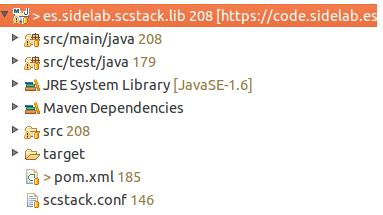
\includegraphics[width=0.5\textwidth]{sidelabcodestack-api-lib}
    \caption{SidelabCode Stack Librería API}
    \label{fig:sidelabcodestack-api-lib}
\end{figure}

\par Para las pruebas del proyecto de la generación del API se ha utilizado en framework \emph{JUnit}\footnote{JUnit - \url{http://junit.org/}}. La cobertura de tests del proyecto en JUnit no es muy halagüeña ya que es del 3,5\%~\ref{fig:sidelabcodestack-sonar} pero en su defensa se puede justificar debido a que se trata de una librería que accede a APIs de terceros. Las APIs o librerías de terceros no han de desarrollar test unitarios sino test test de aprendizaje por lo que no son tan útiles~\cite{clean-code}.

\par Por parte de la publicación del API como servicio Web REST se ha utilizado framework Restlet pero en este caso vemos que la cobertura de test es del 0\%~\ref{fig:sidelabcodestack-sonar-rest-service}. A partir de un proyecto nuevo y dependiente que utiliza la libraría API para publicarla como Servicio Web REST ofreciendo las funcionalidades a la Consola de Administración de la Forja.

\par He utilizado la herramienta \emph{SonarQube}\footnote{SonarQube - \url{http://www.sonarqube.org/}} para obtener una visión más empírica del estado de la cobertura del proyecto. Utilizando las reglas básicas para poder fijarnos en la cantidad de pruebas definidas para SidelabCode Stack \emph{API Lib}~\ref{fig:sidelabcodestack-sonar} y \emph{REST Services}~\ref{fig:sidelabcodestack-sonar-rest-service} ya que para obtener este dato no hace falta un gran refinamiento en la configuración.

\begin{figure}[H]
    \centering
    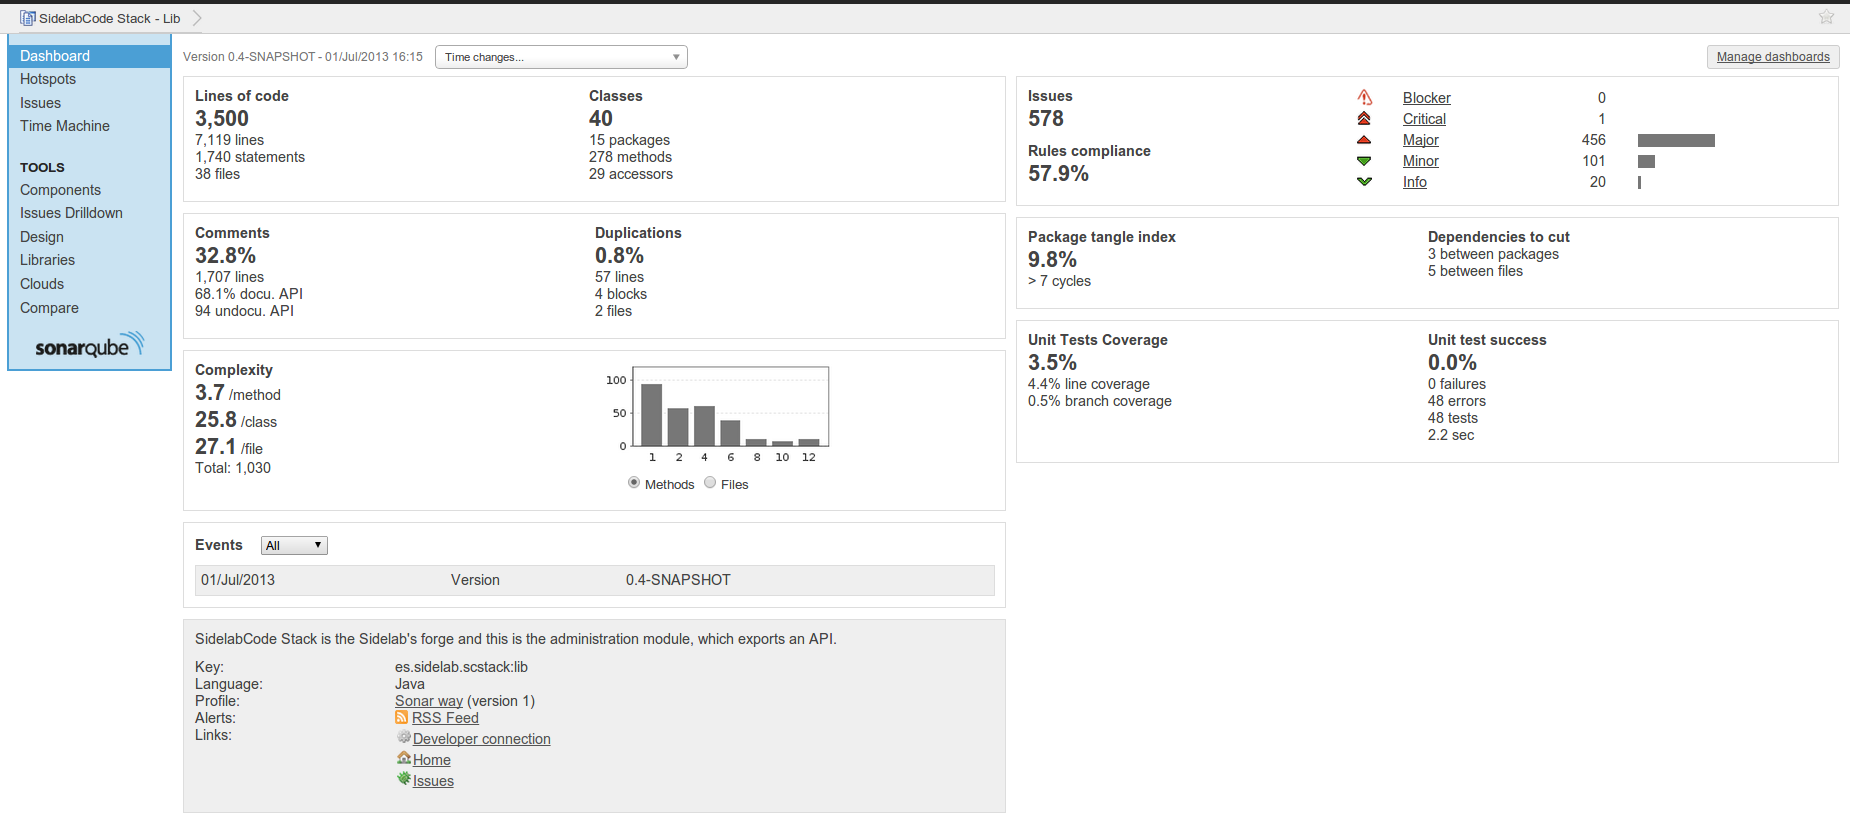
\includegraphics[width=\textwidth]{sidelabcodestack-sonar}
    \caption{SidelabCode Stack API lib Análisis de cobertura con Sonar}
    \label{fig:sidelabcodestack-sonar}
\end{figure}

\begin{figure}[H]
    \centering
    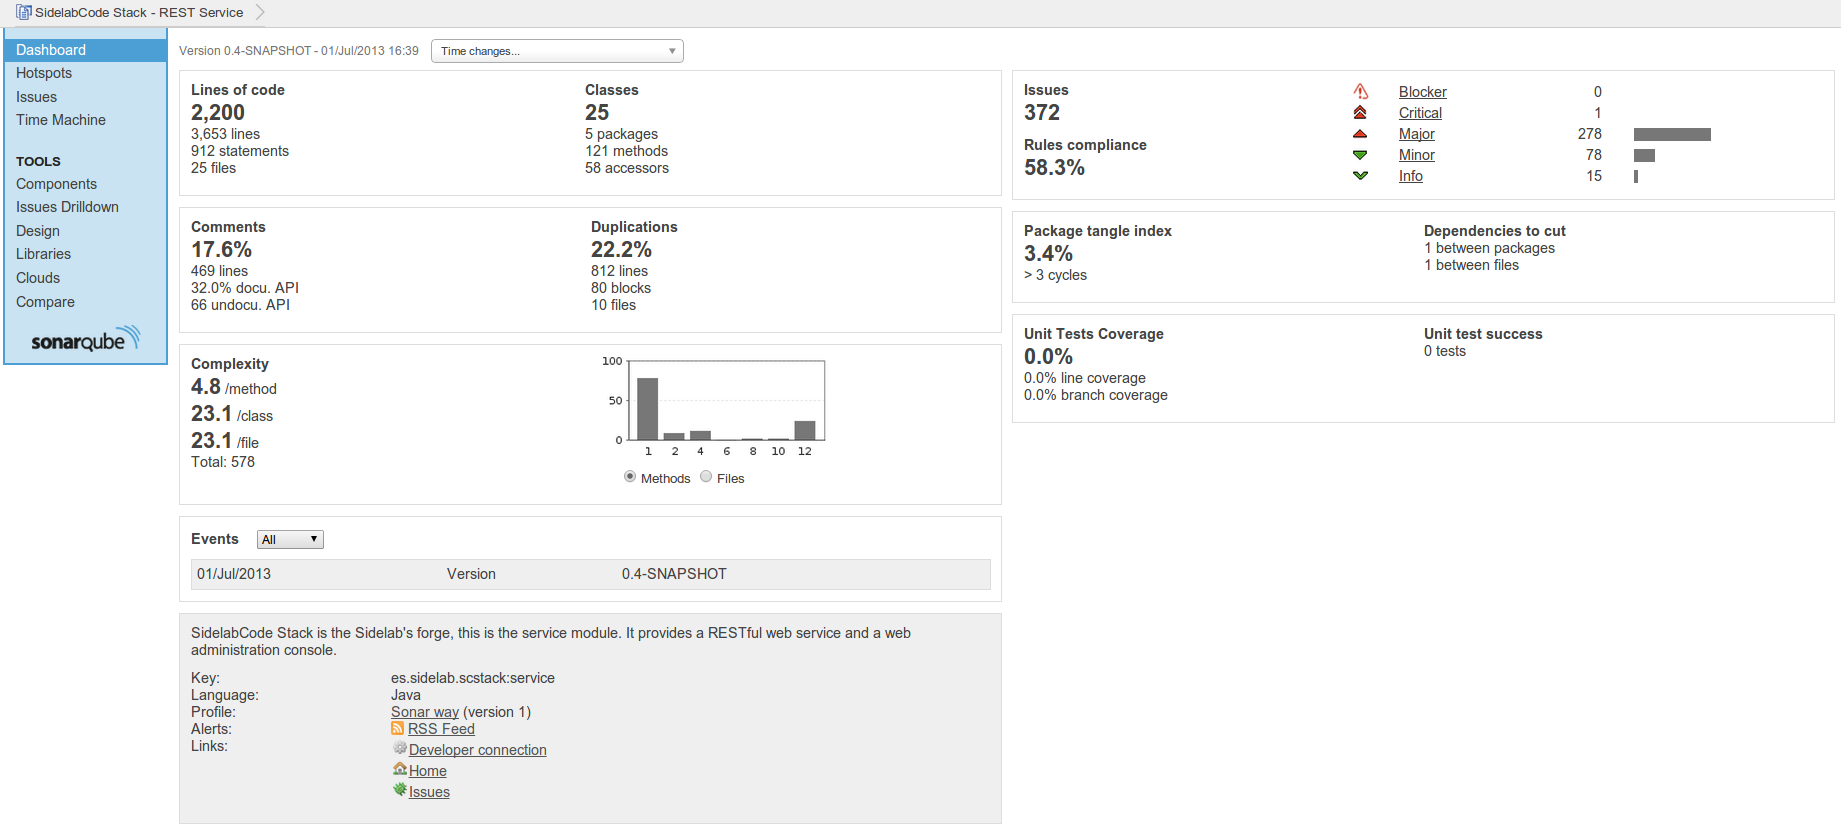
\includegraphics[width=\textwidth]{sidelabcodestack-sonar-rest-service}
    \caption{SidelabCode Stack REST Service Análisis de cobertura con Sonar}
    \label{fig:sidelabcodestack-sonar-rest-service}
\end{figure}

\subsection{Pruebas instalación}
\label{sub:pruebas-instalacion}

\par Las pruebas más importantes en el proceso de desarrollo de la forja SidelabCodeStack han sido las de instalación y configuración de la forja que es donde se encuentra el valor del proyecto. 

\par Previamente a la versión de la forja 0.2 la instalación se ejecutaba a partir de un instalador Java y en consecuencia las pruebas y la replicación de los errores en diferentes entornos acarreaban un trabajo que no podía asumirse con sencillez. A partir de la citada versión (0.2) se introdujo Puppet como herramienta de aprovisionamiento y configuración de los distintos módulos que componen la forja. Este framework ofrece un nuevo camino dentro de las pruebas en el proceso de desarrollo, \emph{la virtualización de las instalaciones}. Puppet nos proporciona un seguimiento completo de la instalación paso a paso a partir de la configuración definida en el proceso. Facilita la ejecución de la instalación de forja en entornos virtuales y seguros para poder asegurar el correcto funcionamiento y descubrir los posibles errores.

\begin{figure}[H]
    \centering
    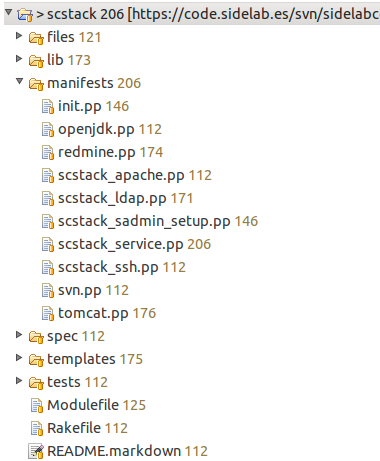
\includegraphics[width=0.5\textwidth]{sctack-puppet}
    \caption{Estructura de módulo Puppet de SCStack}
    \label{sctack-puppet}
\end{figure}

\par Pero no, no es suficiente ya que este manera el desarrollador ha de estar preocupado de invertir el tiempo en la gestión de las distintas máquinas virtuales, asignando espacio, potencia, configuración inicial, sobrecarga de la máquina de desarrollo y cumplir con una serie de tareas repetitivas que le alejan del camino marcado, el proyecto SidelabCode Stack.

\par En este punto aparece \emph{Vagrant}\footnote{Vagrant - \url{http://www.vagrantup.com/}}.

\begin{figure}[H]
    \centering
    
\includegraphics[width=0.3\textwidth]{vagrant}
    \caption{Vagrant Logo}
    \label{fir:vagrant}
\end{figure}

\begin{quote}
    \emph{Create a single file for your project to describe the type of machine you want, the software that needs to be installed, and the way you want to access the machine. Store this file with your project code.}
\end{quote}

\par Vagrant proporciona la gestión de los entornos de desarrollo sobre máquinas virtuales, ligeras, sencillas y replicables. Existe un repositorio de imágenes de virtuales\footnote{VagrantBox.es - \url{http://www.vagrantbox.es/}} preparadas para Vagrant que se han de instalar la máquina del desarrollador con un simple comando:

\lstset{style=bashbasico}
\begin{lstlisting}[frame=trbl]
config.vm.box = "precise64"
config.vm.network :hostonly, "192.168.33.10" # Si se desea se puede utilizar el modo bridge y asignar una ip por dhcp a la maquina dentro de la red en la que se encuentra el host
config.vm.provision :puppet, :module_path => "modules"
\end{lstlisting}

\par Se puede afirmar que Vagrant es la navaja suiza para las pruebas en este proyecto. A través de Vagrant se define el sistema operativo a instalar, la capacidad de la máquina y lo más importante: el \textbf{provisionador}, en nuestro caso Puppet y el módulo SidelabCode Stack.

\par A través de dos comandos se inicia el proceso completo de la instalación de SCStack en una nueva máquina virtual a partir de la configuración de una plantilla con las propiedades necesarias (Apéndice ~\ref{app:instalacion-sidelab}).

\lstset{style=bashbasico}
\begin{lstlisting}[frame=trbl]
$ vagrant box add base http://files.vagrantup.com/precise64.box
$ vagrant init
$ vagrant up
\end{lstlisting}

\par Permite la ejecución de pruebas para la instalación de SCStack de una manera eficiente y controlada aunque también es pesada debido a las características del proyecto.

\par De esta forma se completa el proceso de desarrollo con respecto a las herramientas y módulos utilizados para el desarrollo de la forja SidelabCode Stack ofreciendo las soluciones y herramientas necesarias para poder facilitar el uso del proceso desarrollo Iterativo e Incremental dentro de un marco seguro y fiable.

% subsection pruebas-instalacion (end)

% section pruebas-validacion (end)
